\chapter{Event Simulation}
\label{chapter:simulation}

\section{The Monte Carlo Approach}

In order to understand rare collision events, experimentalists must be able to sort through trillions of collisions to find perhaps only a handful of interesting candidates.  Resolving these events would be impossible without firm theoretical predictions to guide us in deciding what exactly to look for.  It is no simple task, however, to map the equations defining the differential cross sections for various processes onto the discrete event structure of experimental data.  To bridge this gap, we generally use ``Monte Carlo'' techniques~\cite{MonteCarloMethod} where a random number generator is interfaced with the equations governing a certain process in order to produce a large number of simulated collision events.

In practice, simulated data may pass through several different programs, with each specialized to emulate a particular aspect of particle collisions.  The first stage is a matrix element calculation which describes the differential cross section for a given \emph{hard scattering} process or for a set of interfering processes with the same initial and final states (such as in Drell-Yan production of leptons, $q\bar{q} \to \ell^+ \ell^-$, which can be mediated by either a photon or a $Z$ boson~\cite{PhysRevLett.25.316}).  If some of the final-state particles from this initial process are short-lived (such as the vector bosons), their decays will be directly handled in the same calculation due to additional interference possibilities.  For particles with finite lifetimes on the scale of a muon or a tau lepton, decays can be decoupled from the calculation and are generally handled at a subsequent stage.  These later-stage programs choose decays according to branching ratios which are derived primarily through measurements from previous experiments.

Another program takes the colored \emph{partons}---quarks and gluons---produced in the hard scattering interaction along with any radiated gluons and describes how they hadronize into colorless composite particles in a \emph{parton showering} process.  Still another program describes the \emph{underlying event} consisting of soft interactions of the \emph{spectator} partons which did not directly participate in the hard scattering. These programs rely on parameterizations tuned first by input from previous colliders extrapolated to LHC energies and later retuned based on data from initial LHC runs~\cite{Moraes:2007rq,springerlink:10.1007/JHEP01(2011)079}.

\section{Parton Distribution Functions}
Hadron colliders cannot be tuned to take advantage of resonant production because collisions take place at the parton level.  Although each proton carries a well-constrained momentum, the distribution of that momentum amongst its constituents is constantly in flux.  As a result, each hard scattering interaction is unique and a computer simulation must seek to faithfully model both individual scattering interactions with the relevant probabilities along with the aggregate behavior of an ensemble of interactions.  Programs simulating hard scattering events are guided by \emph{parton distribution functions} (PDFs) which describe the relative probability for each parton type to be carrying a particular momentum fraction $x$.  Current calculative ability in QCD is insufficient to predict these distributions, so they are measured experimentally by fits to deep inelastic scattering, production of electroweak bosons, and high energy jet events as well as measurements directly dedicated to determining the strong coupling constant $\alpha_\text{s}$~\cite{CTEQ,MRST}.

\section{Hard Scattering}
The random number generator of a Monte Carlo program is used first to sample a chosen PDF in order to determine an event's initial state and then again to sample the differential cross section, defining momenta for the final state particles. Generators may consider a variety of Feynman diagrams, generally limited to leading order or next-to-leading order contributions, though specialized programs may be used to determine higher-order effects for specific processes when necessary.  Often, a separate program will be used to determine the overall or differential cross section for a process to higher order and these results will be used to apply weighting factors, avoiding the computational expense of running the full calculation for every simulated event.

\section{Parton Showering}

Due to the notion of asymptotic freedom in strong interactions, successful calculations using perturbative QCD can only be valid at very short length scales or very high energies.  These calculations are sufficient to give a good picture of hard scattering interactions at the \TeV scale, but fail to 
consider what happens to the colored partons created in hard interactions or the lower energy interactions which accompany a collision event.  Typically, we would not expect an event containing only the desired state of interest in an analysis; rather, events of interest are accompanied by dozens of low energy hadrons.

A significant fraction of this hadronic activity is due to the energetic colored partons produced from the hard scattering interaction which subsequently shed their energy through parton showers.  Because the energy scale of these showers falls outside the domain of perturbative QCD, we rely instead on a phenomenological description.  In the Lund string model~\cite{Andersson198331}, quarks are bound together with a taught gluon string.  For a pair of quarks travelling away from one another, this string becomes stretched and stores energy, eventually snapping to produce new $q\bar{q}$ pairs when the requisite threshold energy is reached.  With repeated stretching and snapping, the energy scale eventually cools to the point that quarks once again form bound states.  This process of an energetic parton progressing to a collection of colorless bound states is known as \emph{hadronization}.  These resulting hadrons are typically collimated along the direction of the initial hard parton, forming a coherent ``jet'' of particles.  In addition, final or initial state partons may radiate additional partons that are energetic enough to form their own distinct jets.

\begin{figure*}
  \centering
  \subbottom{
    %\documentclass[a4paper,10pt]{book}
%\usepackage{tikz}
%\usetikzlibrary{trees}
%\usetikzlibrary{decorations.pathmorphing}
%\usetikzlibrary{decorations.markings}

%\include{macros}

%\begin{document}


	\begin{tikzpicture}[
					thick,
			% Set the overall layout of the tree
			level/.style={level distance=2.0cm, line width=0.4mm},
			level 2/.style={level distance=2.0cm},
			level 3/.style={level distance=2.0cm},
			level 4/.style={level distance=1.4cm, sibling angle=60}
	]
	%% quark and gluon tree
		\coordinate
			child[grow=-30]{
				child[grow=east] {
					child[grow=60,level distance=1cm] {
						child[grow=20] {
							child[grow=60 , level distance=2.5cm] {
								edge from parent [gluon]	
							}
							child[grow=10] {
								edge from parent [gluon]
							}
							edge from parent [gluon]
						}
						child[grow=60,level distance=4cm] {
							edge from parent [fermion]
						}
						edge from parent [fermion]
					}
					child[grow=-60,level distance=1cm] {
						child[grow=10,level distance=3.5cm] {
							edge from parent [gluon]
						}
						child[grow=-60,level distance=1cm] {
							child[grow=0,level distance=2cm] {
								child[grow=40,level distance=1.2cm] {
									edge from parent [fermion]
		   							node[right=10pt] (p3) {}	
								}
								child[grow=-40,level distance=1cm] {
									edge from parent [fermion]
		   							node[right=5pt] (p1) {}	
								}
								edge from parent [gluon]
							}
							child[grow=-65,level distance=2cm] {
								edge from parent [fermion]
		   						node[right=10pt,below=25pt] (p2) {}	
							}
							edge from parent [fermion]
						}
						edge from parent [fermion]
					}
					edge from parent [boson]
		   			node[above=3pt] {}           
		 		}
				child[grow=210] {
		   			edge from parent [fermion]
		   			node[below=3pt] {}
		 		}
		 		edge from parent [fermion] node [above=3pt] {}
			};

%%Proton and hard interaction	
		\draw[jblue,very thick,decoration={markings,mark=at position 1 with {\arrow[draw=jblue]{>}}}] (-1,0.15) -- (2,0.15) ;
		\draw[jblue,very thick,decoration={markings,mark=at position 1 with {\arrow[draw=jblue]{>}}}] (-1,0) -- (2,0) ;
		\draw[jblue,very thick,decoration={markings,mark=at position 0 with {\arrow[draw=jblue]{>}}}] (-1,-0.15) -- (2,-0.15) ;
		\draw[jblue,very thick,decoration={markings,mark=at position 0 with {\arrow[draw=jblue]{>}}}] (-1,-1.85) -- (2,-1.85) ;
		\draw[jblue,very thick,decoration={markings,mark=at position 0 with {\arrow[draw=jblue]{>}}}] (-1,-2) -- (2,-2) ;
		\draw[jblue,very thick,decoration={markings,mark=at position 0 with {\arrow[draw=jblue]{>}}}] (-1,-2.15) -- (2,-2.15) ;
		\draw[korange,very thick]			(0,0)  circle (0.3cm);
		\fill[kyelloworange,very thick]	(0,0)  circle (0.3cm);
		\draw[korange,very thick]			(0,-2)  circle (0.3cm);
		\fill[kyelloworange,very thick]	(0,-2)  circle (0.3cm);
	
%% Arrows from blobs
		\draw[jblue,very thick,->] (8,-2) -- (9,-1.8) ;
		\draw[jblue,very thick,->] (7.8,-1.5) -- (8.8,-1.3) ;
		
		\begin{scope}[shift={(7.5,0)}]
		\coordinate
			child[grow=10,level distance=0.8cm]{
				child[grow=20,level distance=0.6cm]{
					child[grow=60,level distance=0.5cm]{	 		
						edge from parent [jblue,very thick,->] 
					}	 		
					child[grow=-30,level distance=0.5cm]{	 		
						edge from parent [jblue,very thick,->] 
					}	 			 		
					edge from parent [jblue,very thick] 
				}	 		
				child[grow=-30,level distance=1cm]{	 		
					edge from parent [jblue,very thick,->] 
				}	 		
				edge from parent [fermion] 
			};
		\end{scope}
		
		\draw[jblue,very thick,->] (7.3,1) -- (8.5,1.2) ;
		\draw[jblue,very thick,->] (7.,1.4) -- (8.2,1.6) ;
		
		\begin{scope}[shift={(6.8,3.)}]
		\coordinate
			child[grow=40,level distance=0.8cm]{
				child[grow=60,level distance=0.5cm]{	
					edge from parent [jblue,very thick,->] 
				}	 		
				child[grow=-20,level distance=0.5cm]{	 		
					edge from parent [jblue,very thick,->] 
				}	 		
				edge from parent [fermion] 
			};
		\end{scope}
		
		\draw[jblue,very thick,->] (6.5,3.5) -- (6.9,3.9) ;

		%%low blobs arrows
		\draw[jblue,very thick,->] (7.,-3.5) -- (7.5,-4.1) ;
		\begin{scope}[shift={(6.5,-3.8)}]
		\coordinate
			child[grow=-50,level distance=0.8cm]{
				child[grow=-60,level distance=0.5cm]{	
					edge from parent [jblue,very thick,->] 
				}	 		
				child[grow=-20,level distance=0.5cm]{	 		
					edge from parent [jblue,very thick,->] 
				}	 		
				edge from parent [fermion] 
			};
		\end{scope}

		\draw[jblue,very thick,->] (5.8,-4.2) -- (6.2,-5.) ;

		
		%% String blobs
		\node[] (p4) at (7.2,2.8){};
		\node[] (p5) at (6,3.6){}  ;
		\path[draw=kpurple,rounded corners=6pt,fill=kpurplelight,rotate=30] (p1) rectangle (p2);%(3cm,10pt);
		\path[draw=kpurple,rounded corners=6pt,fill=kpurplelight,rotate=100] (p3) rectangle (p4);%(3cm,10pt);
		\path[draw=kpurple,rounded corners=6pt,fill=kpurplelight,rotate=130] (p4) rectangle (p5);%(3cm,10pt);

	\node[] at (0.0, -3.0) {PDF};
	\node[] at (2.8, -3.0) {Hard scatter};
	\node[] at (5.7, -0.6) {Parton shower};
	\node[] at (8.7, -2.7) {Hadronization};
	\node[] at (10., -0.9) {Decay};

		\end{tikzpicture}
		
		
	%	\end{document}
		
		
		
  }
  \subbottom{
    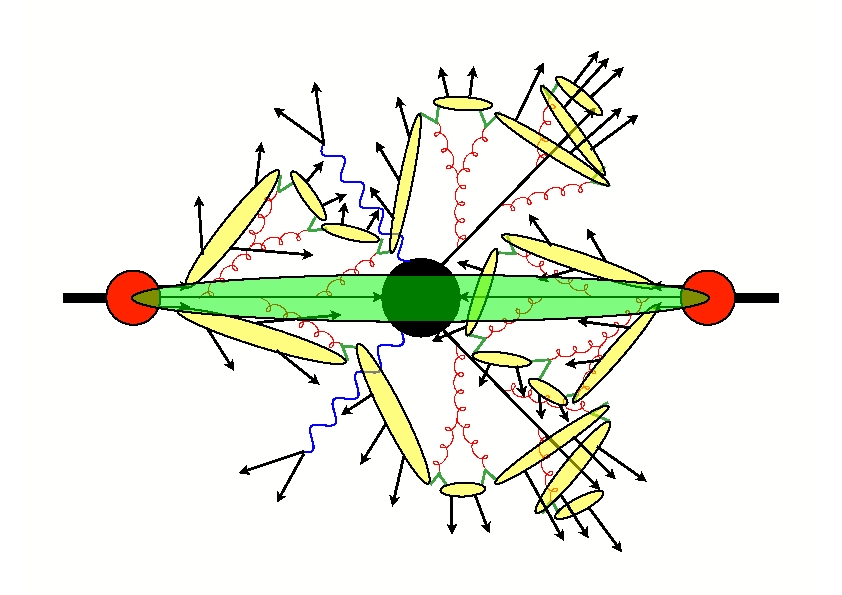
\includegraphics[width=\plotwidth]{figures/mc-schematic.jpg}
  }
  \caption[Two illustrations of a collision event]{Two illustrations of a collision event.  The first (reproduced from~\cite{Grogg:1376067}) is a simplified schematic showing the hard scattering interaction, parton shower, hadronization, and subsequent particle decays.  The second (reproduced from~\cite{Webber:2011}) gives a more complete picture with the hard scatter in green and the hadronization processes in yellow.}
  \label{diagram-showering}
\end{figure*}

\section{Underlying Event}

In addition to the parton showers originating from the hard interaction and from partons radiated in the initial or final state, soft radiation from the remaining partons must also be considered for a full picture of the event.  Because the partons originally formed a colorless proton, this soft radiation will be necessarily connected to the hard partons via a color field, influencing the color and distribution of new $q\bar{q}$ pairs pulled from the vacuum in order to conserve color charge.  The result is a large number of low energy hadrons distributed between the proton remnant and the hard jets which resulted from the final state partons.  This additional activity, known as the \emph{underlying event}, can deposit significant energy in the detector and must be modeled at the hadronization step.

\section{Pileup Interactions}

At LHC luminosities, we are not given the luxury of considering single events independently.  With thousands of protons in each bunch, there are often dozens of collisions in a single crossing.  For simulated events, we copy this effect by superimposing some number of soft interaction events on top of each nominal event, following the interaction multiplicity distribution observed in the experimental data as shown in Fig.~\ref{fig:pileup}.

\begin{figure}
  \centering
  \includegraphics[width=\plotwidth]{matplotlib/pileup/pileup}
  \caption[Distribution of the reconstructed collision vertex multiplicity observed in the 2011 data]{Distribution of the reconstructed collision vertex multiplicity observed in the 2011 data, demonstrating the magnitude of pileup effects.}
  \label{fig:pileup}
\end{figure}


\section{Detector Simulation}

The simulation steps discussed to this point cover only the initial evolution of the system within the vacuum of the beampipe.  As stable or long-lived particles produced in the hard scattering and hadronization processes travel outward from the collision point, they begin to interact with the material of the detector.  A detailed description of the CMS detector and magnetic field is used as input to the \GEANTfour package~\cite{Agostinelli2003250,Allison1610988}, a software toolkit for simulating the passage of particles through matter.  The software simulates not only the decays of the particles as they propagate through various materials, but also the interaction of those particles with the material and the response of the detector to the presence of those particles.  From that response, we simulate signals in the electronics to generate raw data in the same format produced by the physical detector.  From this point on, both collision data and Monte Carlo simulated events can be run through the same reconstruction and analysis software, maximizing the validity of comparisons between them. 


\section{Samples Produced}
\label{sec:mc-samples}
For all Monte Carlo samples considered in this analysis, a matrix element generator is interfaced with \PYTHIA~\cite{PYTHIA} which handles hadronization and then to \TAUOLA~\cite{Was:2000st} which handles all tau decays.  The CMS collaboration handles sample generation centrally whenever possible as a means to ensure consistency in configuration.  Except for our \wprime signal, we use official samples which have been configured to match the beam energy, detector conditions, and luminosity distribution of the full sample of collision data taken in 2011.

\begin{table}
\centering
\newcommand{\mymass}[1]{\makebox[\widthof{0000}][r]{#1}}
\newcommand{\mysigma}[1]{\makebox[\widthof{\num{1.000e-1}}][l]{\num{#1}}}
\begin{tabular}{ c c c c }
  \toprule
  $M(\wprime)c^2/\GeV$ & $\sigma_\mathrm{LO}/\pb$ & $\sigma_\mathrm{NNLO}/\pb$ & $k$\\
  \midrule
  \mymass{ 200} & \mysigma{1.324e0 } & \mysigma{1.797e0 } & 1.357\\
  \mymass{ 250} & \mysigma{1.118e0 } & \mysigma{1.517e0 } & 1.357\\
  \mymass{ 300} & \mysigma{6.337e-1} & \mysigma{8.599e-1} & 1.357\\
  \mymass{ 400} & \mysigma{2.040e-1} & \mysigma{2.768e-1} & 1.357\\
  \mymass{ 500} & \mysigma{7.915e-2} & \mysigma{1.074e-1} & 1.357\\
  \mymass{ 600} & \mysigma{3.620e-2} & \mysigma{4.890e-2} & 1.351\\
  \mymass{ 700} & \mysigma{1.806e-2} & \mysigma{2.440e-2} & 1.352\\
  \mymass{ 800} & \mysigma{9.857e-3} & \mysigma{1.328e-2} & 1.347\\
  \mymass{ 900} & \mysigma{5.551e-3} & \mysigma{7.440e-3} & 1.341\\
  \mymass{1000} & \mysigma{3.322e-3} & \mysigma{4.420e-3} & 1.332\\
  \mymass{1100} & \mysigma{2.041e-3} & \mysigma{2.704e-3} & 1.325\\
  \mymass{1200} & \mysigma{1.289e-3} & \mysigma{1.690e-3} & 1.311\\
  \mymass{1300} & \mysigma{8.333e-4} & \mysigma{1.082e-4} & 1.298\\
  \mymass{1400} & \mysigma{5.395e-4} & \mysigma{6.900e-4} & 1.279\\
  \mymass{1500} & \mysigma{3.606e-4} & \mysigma{4.560e-4} & 1.265\\
  \bottomrule
\end{tabular}
\caption[Cross sections of \wprime{} signal samples]{An overview of the $W' \to WZ \to \ell\nu\ell\ell$ signal samples considered in this analysis, giving the \wprime mass along with the associated leading order (LO) and next-to-next-to-leading order (NNLO) cross sections in the SSM followed by the associated $k$-factor. These samples were locally produced, following the same prescription used for official samples.  The cross sections include the branching ratios for the bosonic decays into charged leptons ($e$, $\mu$, or $\tau$).}
\label{tab:signalsampleinfotable}
\end{table}

\begin{table}
\centering
\newcommand{\mysigma}[1]{\makebox[\widthof{\num{1.000e-1}}][l]{\num{#1}}}
\newcommand{\mubox}[1]{\makebox[\widthof{$\mu$}][c]{$#1$}}
\newcommand{\zzto}[2]{\ensuremath{ZZ \to \mubox{$#1$}^+ \mubox{$#1$}^- \mubox{$#2$}^+ \mubox{$#2$}^-}}
\begin{tabular}{ c r c c }
  \toprule
  & Sample & $\sigma_\mathrm{LO}/\pb$ & $\sigma_\mathrm{(N)NLO}/\pb$ \\
  \midrule
  \multirow{6}{\baselineskip}{\begin{sideways}\parbox{18mm}{\MADGRAPH}\end{sideways}}
  & $WZ(\to \ell\nu\ell\ell)\,+$ jets & \mysigma{7.19e-1} & \mysigma{8.79e-1} \\ 
  & $WW(\to \ell \nu \ell \nu)\,+$ jets & \mysigma{3.78e0} & \mysigma{4.89e0} \\
  & $Z(\to\ell\ell)\,+$ jets &  \mysigma{2.47e3} & \mysigma{3.05e3} \\ 
  & $W(\to\ell\nu)\,+$ jets & \mysigma{2.78e4} & \mysigma{3.13e4} \\ 
  & $V\gamma\, +$ jets & \mysigma{1.73e2} & ---  \\ 
  & $t\bar{t}\,+$ jets & \mysigma{9.48e1} & \mysigma{1.58e2} \\ 
  \midrule
  \multirow{6}{\baselineskip}{\begin{sideways}\parbox{15mm}{\POWHEG}\end{sideways}}
  & \zzto{$e$}{$e$} & --- & \mysigma{1.54e-2} \\
  & \zzto{$\mu$}{$\mu$} & --- & \mysigma{1.54e-2} \\
  & \zzto{$\tau$}{$\tau$} & --- & \mysigma{1.54e-2} \\
  & \zzto{$e$}{$\mu$} & --- & \mysigma{3.08e-2} \\
  & \zzto{$e$}{$\tau$} & --- & \mysigma{3.08e-2} \\
  & \zzto{$\mu$}{$\tau$} & --- & \mysigma{3.08e-2} \\
  \bottomrule
\end{tabular}
\caption[Cross sections of background samples]{Background processes considered for this analysis with leading order (LO) and higher-order cross sections.  Each process corresponds to a dataset from official production, using either \MADGRAPH or \PYTHIA for the matrix element calculation. The $W\,+$ jets cross section is next-to-next-to-leading order (NNLO) while all others are next-to-leading order (NLO).  The $V\gamma\,+$ jets sample considers both of the heavy vector ($V$) bosons $W$ and $Z$.}
\label{tab:sampleinfotable}
\end{table}

\subsection{Backgrounds}
All simulated background samples are taken from official production of Monte Carlo events (see Table~\ref{tab:sampleinfotable}).  The matrix element calculation is handled by either \MADGRAPH~\cite{MADGRAPH} or \POWHEG~\cite{POWHEG}, both programs which operate to fixed order in $\alpha_\text{s}$, generating a given electroweak final state with additional jets.  Where possible, we replace this fixed-order cross section with a value obtained from a higher-order calculation using a generator or dedicated program within the same phase space and parameters.

Our primary background for a resonant search is SM $WZ$ production.  The $WZ$ Monte Carlo events are generated with \MADGRAPH while the cross section is taken from MCFM~\cite{Campbell:2011bn}.  We must also consider $ZZ$ production as an irreducible background where one of the leptons is either outside detector acceptance or is misreconstructed.  The other backgrounds represent reducible processes that can be confused with signal due to misidentified lepton candidates from jets and photons.  We expect these events with jets faking leptons to be a significant concern, so we pay special attention that the jets are well-modeled in the Monte Carlo.  \MADGRAPH is designed with such needs in mind and includes diagrams with up to four jets in addition to the base process for which it is configured.  This treatment, coupled with an accurate model of parton showering and the detector's response to jet activity, allows CMS to model the probability that jets are misreconstructed as charged leptons.

\subsection{Signal}
Both \wprime and Technicolor models are implemented in the current version of \PYTHIA.  The current implementation of LSTC which corresponds to the Technicolor parameter space of interest for this study, however, contains errors leading to an artificially low fraction of longitudinally polarized technihadrons.  Because the expected kinematics for \technirho{} events in the LSTC are quite similar to those for SSM \wprime, the \PYTHIA \wprime routines can also serve as a sufficient model for Technicolor events.  

Although \PYTHIA considers only leading order diagrams in its matrix element calculations, we can apply a scaling factor to the results in order to bring the overall cross section in line with a higher-order calculation.  For all signal samples, we employ an NNLO calculation from MCFM which includes all diagrams of order $\alpha_\text{s}$ as well as the ``box diagram'' for $WZ$ radiation initiated from a pair of gluons, which is of order $\alpha_\text{s}^2$.

For the \wprime search, we focus on fifteen individual mass points between \simass{200} and \simass{1500}, in each case producing \num{20000} events in \PYTHIA and an NNLO cross section in MCFM
(see Table~\ref{tab:signalsampleinfotable}).  
For Technicolor investigations, we use these same \wprime samples from \PYTHIA, but apply modified cross sections.  Each sample is assigned a leading order cross section from the \PYTHIA LSTC implementation which is then scaled by a factor $\sigma_\text{NNLO}/\sigma_\text{LO}$ (known as a $k$-factor) determined from the MCFM calculations for \wprime (see Table~\ref{tab:technicolorgen}).

% COMMENT:
% Technically NLO means including diagrams for process with the same 
% final states that take place at higher order due to loops.
% Commonly in the field NLO means including diagrams with the same electroweak
% final state particles and additional jets due to QCD radiation.  When your read
% about an NNLO cross section predictions for WZ production what they are
% really talking about is including final states with up to two jets.   
% The order they are talking about is actually the order of the strong
% coupling constant beyond the order in alpha_s necessary to produce the
% basic electroweak final state.  Also often included in an NNLO calculation 
% will also be loop diagrams to the same order in alpha_s.  So for WZ production
% an NNLO calculation would include WZ, WZ+1jet, WZ+2jets, WZ produced via
% gluons to a box diagram(two strong vertices) with the WZ radiated off of
% the other side of the box.  Note that sometimes the last is not included
% because it is technically very difficult.  Sometimes they will include
% diagrams with extra electroweak couplings, but typically not because
% every electroweak vertex has an on order 1/137 suppression and the
% addition to the cross section is small.  Also sometimes a cross section
% calculation will include an attempt to resum all higher order effects
% (resummation) after the NNLO treatment to improve the final result.  That
% is why you would want to normalize to that number to improve the result.


\begin{table*}[!h]
  \centering
  \begin{tabular}{c c c c c c}
    \toprule
    $M(\technirho)$ & $M(\technia)$ & $M(\technipi)$ & $(\sigma_\text{LO} \times \text{BR})/\pb$ & $(\sigma_\text{NNLO} \times \text{BR})/\pb$ \\
    \midrule
    200 & 220 & 125 & \num{3.872e-1} & \num{5.254e-1} \\ %            
    250 & 275 & 163 & \num{2.144e-1} & \num{2.909e-1} \\ %            
    300 & 330 & 200 & \num{9.616e-2} & \num{1.305e-1} \\ %\num{42.74} 
    400 & 440 & 275 & \num{2.889e-2} & \num{3.920e-2} \\ %\num{12.84} 
    500 & 550 & 350 & \num{1.172e-2} & \num{1.590e-2} \\ %\num{5.208} 
    600 & 660 & 425 & \num{5.612e-3} & \num{7.582e-2} \\ %\num{2.494} 
    700 & 770 & 500 & \num{2.943e-3} & \num{3.979e-3} \\ %\num{1.308} 
    800 & 880 & 575 & \num{1.670e-3} & \num{2.249e-3} \\ %\num{0.742} 
    900 & 990 & 650 & \num{9.740e-4} & \num{1.306e-3} \\ %\num{0.432} 
    \bottomrule
  \end{tabular}
  \caption[Technicolor parameters used for cross section generation]{Technicolor parameters used to generate cross sections for this analysis.  All masses are given in \GeVcc.  BR refers to the product of the branching ratios of the \technirho/\technia to $WZ$ and the subsequent decay of $W$ and $Z$ to electrons, muons, or taus.  Quoted cross sections are computed by \PYTHIA to leading order (LO).}
  \label{tab:technicolorgen}
\end{table*}

For Technicolor, we concentrate on the TCSM mass points not excluded by other experiments which cover a phase space region accessible with \SI{5}{\fbinv} of data.  As discussed in Section~\ref{sec:technicolor}, suppression of the electroweak $S$ parameter requires near degeneracy between the vector and axial-vector resonances; we choose $M(\technia) = 1.1 M(\technirho)$.

The relationship between $M(\technirho)$ and $M(\technia)$ significantly affects $\text{BR}(\technirho \to WZ)$.  The $WZ$ branching ratio drops below 10\% for $M(\technirho) > M(\technipi)$, but approaches unity if $M(\technirho) < M(\technipi) + M(W)$.  For this analysis, we assume a parameter set used in previous CMS investigations~\cite{Brooijmans:2010tn} where $M(\technipi) = \frac{3}{4} M(\technirho) - 25\GeV$ and also investigate the dependence of the results on the relative values of the \technirho and \technipi masses.
